\documentclass[a4paper,english,12pt]{article}
\usepackage{%
	amsfonts,%
	amsmath,%	
	amssymb,%
	amsthm,%
	babel,%
	bbm,%
	biblatex,%
	caption,%
	centernot,%
	color,%
	enumerate,%
	%enumitem,%
	epsfig,%
	epstopdf,%
	etex,%
	framed,%
	fullpage,%
	geometry,%
	graphicx,%
	hyperref,%
	latexsym,%
	mathptmx,%
	mathtools,%
	multicol,%
	pgf,%
	pgfplots,%
	pgfplotstable,%
	pgfpages,%
	proof,%
	psfrag,%
	subfigure,%	
	tikz,%
	times,%
	ulem,%
	url,%
	xcolor%
}	
\definecolor{shadecolor}{gray}{.95}%{rgb}{1,0,0}
\usepackage[mathscr]{eucal}
\usepgflibrary{shapes}
\usetikzlibrary{%
  arrows,%
  backgrounds,%
  chains,%
  decorations.pathmorphing,% /pgf/decoration/random steps | erste Graphik
  decorations.text,%
  matrix,%
  positioning,% wg. " of "
  fit,%
  patterns,%
  petri,%
  plotmarks,%
  scopes,%
  shadows,%
  shapes.misc,% wg. rounded rectangle
  shapes.arrows,%
  shapes.callouts,%
  shapes%
}

\theoremstyle{plain}
\newtheorem*{thm*}{Theorem}
\newtheorem*{exmp*}{}
\newtheorem{thm}{Theorem}[section]
\newtheorem{lem}[thm]{Lemma}
\newtheorem{prop}[thm]{Proposition}
\newtheorem{cor}[thm]{Corollary}

\theoremstyle{definition}
\newtheorem{defn}[thm]{Definition}
\newtheorem{conj}[thm]{Conjecture}
\newtheorem{exmp}[thm]{Example}
\newtheorem{assum}[thm]{Assumptions}
\newtheorem{axiom}[thm]{Axiom}

\theoremstyle{remark}
\newtheorem{rem}[thm]{Remark}
\newtheorem{note}[thm]{Note}
\newtheorem{con}[thm]{Construction}

\newcommand{\eq}[1]{\begin{align*}#1\end{align*}}
\newcommand{\eqn}[1]{\begin{align}#1\end{align}}
\newcommand{\EQ}[1]{\begin{equation*}#1\end{equation*}}
\newcommand{\EQN}[1]{\begin{equation}#1\end{equation}}
\newcommand{\meq}[2]{\begin{xalignat*}{#1}{#2}\end{xalignat*}}
\newcommand{\meqn}[2]{\begin{xalignat}{#1}{#2}\end{xalignat}}
\newcommand{\norm}[1]{\left\lVert#1\right\rVert}
\newcommand{\indep}{\!\perp\!\!\!\perp}
\DeclarePairedDelimiter\abs{\lvert}{\rvert}%
%\DeclarePairedDelimiter\norm{\lVert}{\rVert}%
\newcommand{\tr}{\operatorname{tr}}
\newcommand{\Var}{\operatorname{Var}}
\newcommand{\Cov}{\operatorname{Cov}}

\newcommand{\D}{\mathbb{D}}
\newcommand{\E}{\mathbb{E}}
\newcommand{\N}{\mathbb{N}}
\newcommand{\Q}{\mathbb{Q}}
\renewcommand{\P}{\mathbb{P}}
\newcommand{\R}{\mathbb{R}}
\newcommand{\Z}{\mathbb{Z}}

\newcommand{\C}{\mathcal{C}}
\newcommand{\cG}{\mathcal{G}}

\newcommand{\sB}{\mathscr{B}}
\newcommand{\sE}{\mathscr{E}}
\newcommand{\sF}{\mathscr{F}}
\renewcommand{\sL}{\mathscr{L}}
\newcommand{\sS}{\mathscr{S}}
\newcommand{\sT}{\mathscr{T}}


\renewcommand{\le}{\leqslant}
\renewcommand{\ge}{\geqslant}

% Debug
\newcommand{\todo}[1]{\begin{color}{blue}{{\bf~[TODO:~#1]}}\end{color}}


\makeatletter
\def\th@plain{%
  \thm@notefont{}% same as heading font
  \itshape % body font
}
\def\th@definition{%
  \thm@notefont{}% same as heading font
  \normalfont % body font
}
\makeatother
\date{}
\usepackage{graphicx}
\graphicspath{ {./figures/} }

%opening
\title{Lecture-05: Kernel Methods}
\date{Aug 16, 2018}
\author{Raj Magesh G}


\begin{document}
\maketitle
\section{Kernel Methods}

\begin{itemize}
	\item Kernel methods are an extension of SVMs to non-linear boundaries.
	\item The algorithm for an SVM depends solely on evaluating inner products of sample points.
	\item A non-linear separation boundary in input space $X$ may be a linear separation in a higher-dimensional space.
\end{itemize}

\section{Introduction}

\[\Phi : \sX \rightarrow H ~~~ \text{is a non-linear map.}\]


\begin{exmp}
\textbf{Document classification}. Let $\sX$ be the set of words in a document, which has a typical size of $|\sX| = 10^5$ words. Classifying the document into different types based on single words (elements from the set $\sX$) will be difficult because many types of documents will share the same words. A better way to classify documents is to look for patterns in groups of adjacent words. For example, consider $\sX^3$, which is the set of trigrams (triplets of words). Classifying documents in the space of trigrams will yield better results despite the increased size of the space $|\sX^3| = 10^{15}$.
\end{exmp}

\begin{rem}
	\textbf{Why do we use kernel methods?}
\begin{itemize}
	\item \textbf{Pros}: Generalization guarantees depend solely on the margin $\rho$ and the number of samples $n$.
	\item \textbf{Cons}: Computation of inner products may be expensive.
\end{itemize}
\end{rem}

\begin{defn}
	A function $K : \sX \times \sX \rightarrow \R$ is called a \textit{kernel} over $\sX$.
\begin{itemize}
	\item For all $x, x' \in \sX$, $K(x, x') = \langle \Phi(x), \Phi(x') \rangle_{H}$ for some mapping $\Phi : \sX \rightarrow H$.
	\item $\langle \cdot, \cdot \rangle$ is a similarity measure between two vectors in feature space $H$.
	\item $K$ is a similarity measure between elements of $\sX$.	
\end{itemize}
\end{defn}

\begin{rem}
	\textbf{Why do we work with kernels?}
\begin{itemize}
	\item \textbf{Efficiency}: Computation in the input space $\sX$ is more efficient than computation in the feature space $H$ because $\text{dim}(H) >> \text{dim}(\sX)$ and $\langle x, y \rangle = O(\text{dim}(\sX))$.
	\item \textbf{Flexibility}: There is no need to explicitly define the map $\Phi$ but its existence is guaranteed if $K$ satisfies certain conditions.
\end{itemize}
\end{rem}

\begin{thm}
	\textbf{Mercer's condition}
	
Let $\sX \subseteq \R^{N}$ be a compact set and let $K: \sX \times \sX \rightarrow\R$ be a continuous and symmetric function. Then, $K$ admits a uniformly convergent expansion of the form
\[K(x,x') = \sum_{n=0}^{\infty} a_n \phi_n(x) \phi_n(x')\]
with $a_n > 0$ iff for any square integrable function $c \in L_2 (x)$, the following condition holds
\[\iint_{\sX \times \sX} c(x) c(x') K(x, x') dx dx' \ge 0\]
which is the positive semi-definiteness of $K$.
\end{thm}

\section{PDS Kernels}

\begin{defn}
	A kernel $K: \sX \times \sX \rightarrow \R$ is \textit{positive definite symmetric (PDS)} if for any $\mathbf{X} \in \sX^{m}$, the matrix $\mathbf{K} = [K(x_i, x_j)]_{ij}$ is \textit{symmetric positive semi-definite (SPSD)}.
\[\mathbf{K} =
\begin{bmatrix}
	K(x_1,x_1) 	& \dots 	& K(x_1, x_m) \\
	\vdots		& \ddots 	& \vdots \\
	K(x_m, x_1) & \dots		& K(x_m, x_m)
\end{bmatrix}
\] 

$\mathbf{K}$ is called the Gram matrix or the kernel matrix associated to a kernel $K$ and sample $S$.
\begin{rem}
	\textbf{Reminder of matrix properties}
	\begin{itemize}
		\item \textbf{Symmetry}: $\mathbf{K}_{ij} = \mathbf{K}_{ji}$
		\item \textbf{Positive semi-definiteness}: $\mathbf{X^T K X} \ge 0$ for all $\mathbf{X} \in \R^m$
	\end{itemize}
\end{rem}
\end{defn}

\begin{exmp}
	\textbf{Polynomial kernel}
	
For $c>0$ and degree $d \in \N$,
\[K(x,x') = (\langle x, x' \rangle + c)^d ~~~ \text{for} ~~~ x,x' \in \sX \subseteq \R^N\]

\textbf{[HW]} For this mapping $\Phi: \sX \rightarrow H$, find the dimension of $H$.

For $N=2$ and $d=2$,
\begin{align*}
K(x,x') &= (x_1 x_1^{'} + x_2 x_2^{'} + c)^2 \\
&= \langle
\begin{bmatrix}
x_1^2 \\
x_2^2 \\
\sqrt{2} x_1 x_2 \\
\sqrt{2c} x_1 \\
\sqrt{2c} x_2 \\
c
\end{bmatrix}
,
\begin{bmatrix}
x_1^{'2} \\
x_2^{'2} \\
\sqrt{2} x_1^{'} x_2^{'} \\
\sqrt{2c} x_1^{'} \\
\sqrt{2c} x_2^{'} \\
c
\end{bmatrix}
\rangle
\end{align*}

Consider the following classification problem shown in Figure 1, where the red and the blue points must be separated by a hyperplane. This is not possible in the space $x_1 \times x_2$ since no separable hyperplane exists. 

\begin{figure}[h]
	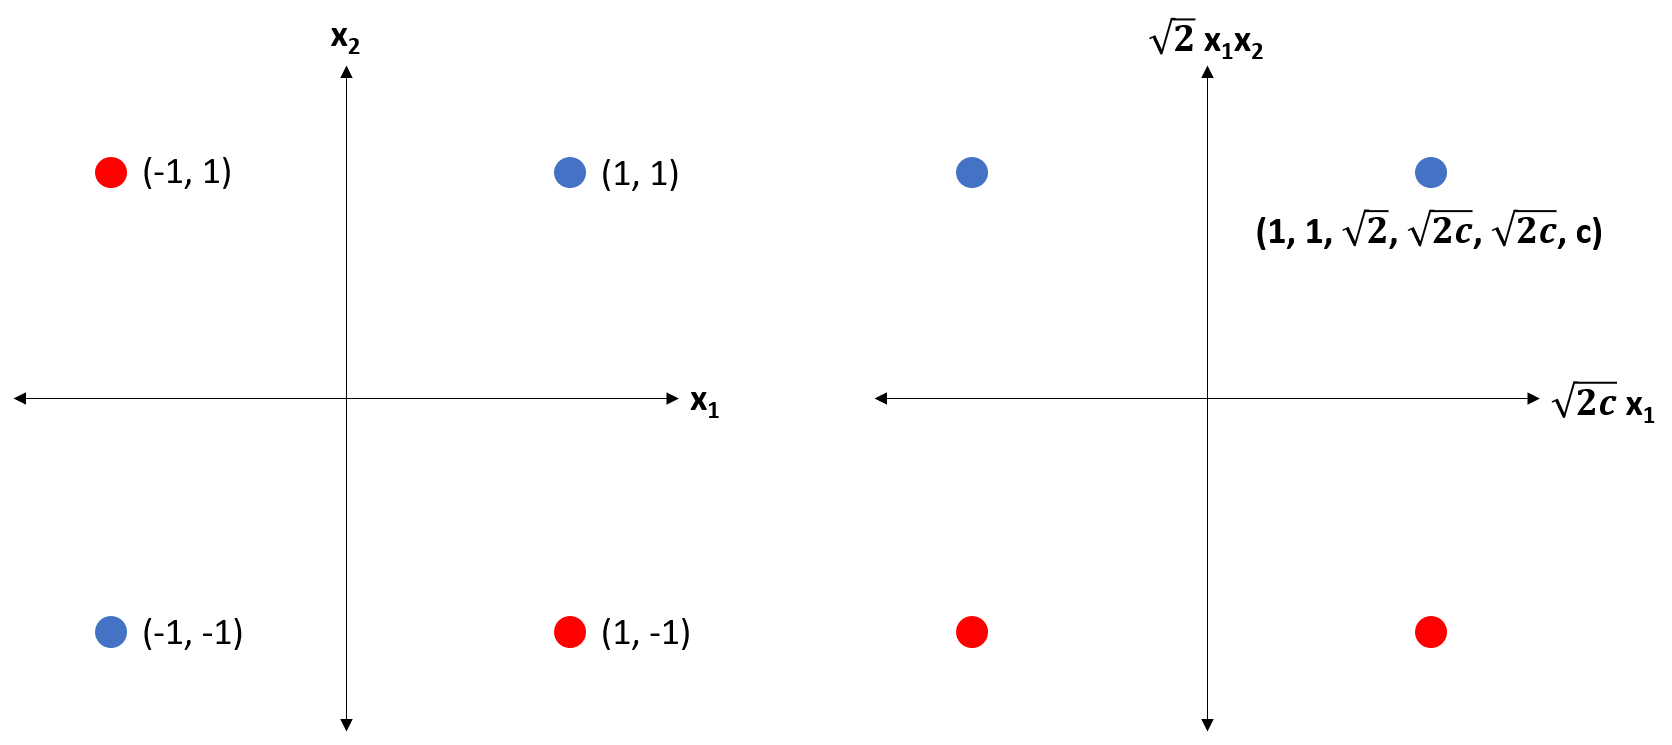
\includegraphics[scale=0.5]{kernel-methods-polynomial-kernel}
	\centering
	\caption{Left: Four points from two classes plotted on the $x_1, x_2$ axes. These points are not separable by any hyperplane. Right: The same four points are plotted on the $\sqrt{2} x_1 x_2$ and $\sqrt{2c} x_1$ axes. These points are now separable.}
\end{figure}
However, when we use the function $h(x_1,x_2) = x_1 x_2$ to bring these points to a higher-dimensional space, we find that these points are indeed separable along the $x_1 x_2$ dimension, as can be seen in Figure 2.

\end{exmp}

\begin{exmp}
	\textbf{Gaussian kernel}

For any $\sigma > 0$, a \textit{Gaussian kernel} is defined as $K: \sX\times\sX\rightarrow\R$ such that
\[K(x,x') = \text{exp}\left(\dfrac{-||x-x'||^2}{2 \sigma^2}\right)\]
This is a PDS kernel derived by normalization of the following kernel
\begin{align*}
K'(x,x') &= \text{exp}\left(\dfrac{\langle x, x' \rangle}{\sigma^2}\right) \\
&= \sum_{n=0}^{\infty} \dfrac{1}{n!}\left(\dfrac{\langle x, x' \rangle}{\sigma^2}\right)^n
\end{align*}
\end{exmp}

\begin{exmp}
	\textbf{Sigmoid kernel}

\[K(x,x') = \tanh(a \langle x,x' \rangle + b) ~~~ \text{for} ~~~ a,b \ge 0\]

This kernel is used in sigmoid perceptrons in neural networks due to its similarity to the sign function.
\end{exmp}

\section{Reproducing Kernel Hilbert Space (RKHS)}

\begin{lem}
	\textbf{Cauchy-Schwarz inequality for PDS kernel}

Let $K$ be a PDS kernel. Then $K^2(x,x') \le K(x,x)K(x',x')$ for all $x, x' \in \sX$.
\end{lem}

\begin{proof}
	\[\mathbf{K} =
	\begin{bmatrix}
	K(x_1,x_1) 	& \dots 	& K(x_1, x_m) \\
	\vdots		& \ddots 	& \vdots \\
	K(x_m, x_1) & \dots		& K(x_m, x_m)
	\end{bmatrix}
	\] $\mathbf{K}$ is a positive semi-definite matrix.
	
	\[K(x,x)K(x',x') \ge K^2(x,x')\]
\end{proof}

\begin{thm}
\textbf{Reproducing Kernel Hilbert Space (RKHS)}

Let $K: \sX \times \sX \rightarrow \R$ be a PDS kernel. Then, there exists a Hilbert space $H$ and a mapping $\Phi: \sX \rightarrow H$ such that for all $x, x' \in \sX$,

\[K(x,x') = \langle \Phi(x), \Phi(x')\ \rangle _H\]

Furthermore, $H$ has the following property known as the reproducing property. For all $h \in H$, $x \in \sX$, $h(x) = \langle(h(\cdot),K(x, \cdot)\rangle$. $H$ is called the RKHS associated with the kernel $K$. 
\end{thm}

\begin{proof}
	For any $x \in \sX$, define $\Phi_x:\sX\rightarrow\R$ such that $\Phi_x(x') = K(x,x')$.
	Let us take $H_0$, the span of finitely many $x_i$s.
	\[H_0 = \left\lbrace \sum_{i \in I}a_i \Phi_{x_i}, a_i \in \R, x_i \in \sX, |I| < \infty\right\rbrace\]
	
	Then, we define a function $\langle \cdot, \cdot \rangle: H_0 \times H_0 \rightarrow \R$ such that
	
	\[\langle f, g \rangle := \sum_{i \in I, j \in J} a_i b_j K(x_i, x_j)\]
	
	where $f = \sum_{i \in I} a_i \Phi_{x_i}$ and $g = \sum_{j \in J} b_j \Phi_{x_j}$.
\end{proof}

\begin{rem} \textbf{Properties of $\langle \cdot, \cdot \rangle$}
\begin{itemize}
		\item \textbf{Symmetry}: By definition, $\langle \cdot, \cdot \rangle$ is symmetric.
		\item $\langle \cdot, \cdot \rangle$ does not depend on the particular representation of $f$, $g$.
		\item \textbf{Bilinearity}: $\langle \cdot, \cdot \rangle$ is bilinear. \textbf{[HW]} Show that $\langle \alpha f + \beta h, g \rangle = \alpha \langle f, g \rangle + \beta \langle f, g \rangle$
		\item \textbf{Positive semi-definiteness}: For $f \in H_0$, $f = \sum_{i \in I} a_i \Phi_{x_i}$ and $\langle f, f \rangle = \sum_{i \in I} \sum_{j \in J} a_i a_j K(x_i,x_j) \ge 0$
		\item For any $f \in H_0$, $x \in \sX$, $\langle f, \Phi_{x_0} \rangle^2 = \left[\sum_{i=1}^m a_i K(x_i, x_0)\right]^2$. \textbf{[HW]} Show that $\langle f, \Phi_{x_0} \rangle^2 \le \langle f, f \rangle \langle \Phi_{x_0}, \Phi_{x_0} \rangle$.
		\item \textbf{Reproducing property}: Let $f \in H_0$ and $f = \sum_{i=1}^m a_i \Phi_{x_i}$. Then, $\langle f, \Phi_x \rangle = \sum_{i=1}^m a_i K(x, x_i) = f(x)$.
		\item $H_0$ is a pre-Hilbert space which can be made complete to form the Hilbert space $H = \overline{H_0}$, where $H_0$ is dense in $H$. 
\end{itemize}
\end{rem}
\end{document}